\chapter{Arhitektura i dizajn sustava}
		
		 Arhitektura sustava zasnivat će se na MVC (Model-View-Controller)
		načelu. Temeljno obilježje ovog obrasca jest podjela aplikacije u 3 međusobno povezane komponente:
		
		\begin{figure}[h]
			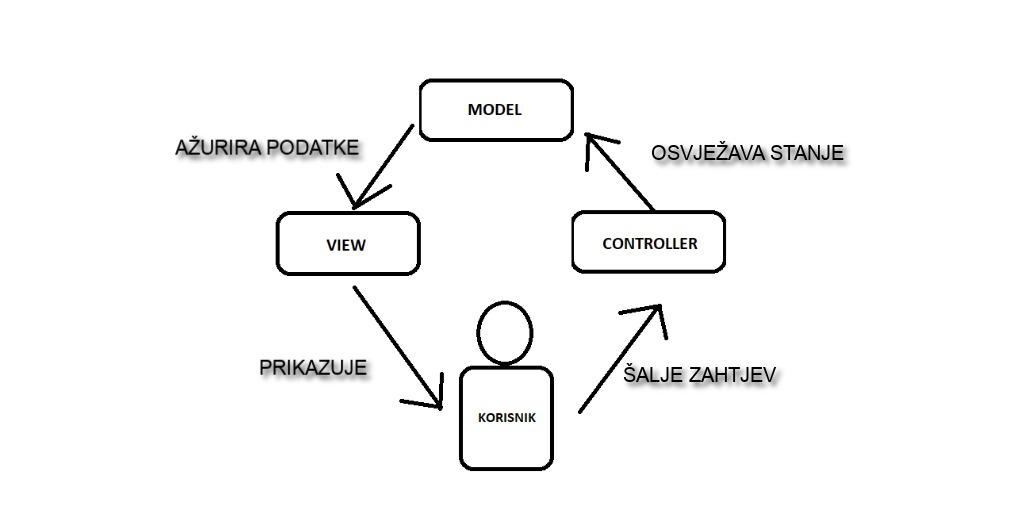
\includegraphics[scale=0.5]{images/mvc.jpeg}
			\caption{MVC načelo}
			\label{fig:MVC slika} 
		\end{figure}
		\begin{itemize}
			\item 	\textit{ \textbf{Model} je centralna komponenta sustava, sadrži podatke te razrede čijim se objektima modelira, .}
			\item 	\textit{\textbf{View} predstavlja prikaz obrađenih podataka.}
			\item 	\textit {\textbf{Controller} upravlja korisničkim zahtjevima te ih prosljeđuje modelu.}
		\end{itemize}
		\paragraph{}
		
		Na ovaj je način korisničko sučelje izdvojeno, čime je automatski smanjena njegova međuovisnost s ostatkom sustava. Upravitelj modelu šalje naredbe i osvježava njegovo stanje dok pogled od modela prikuplja informacije koje potom predstavlja korisniku.  
		
		\paragraph{}
		
		Za razvoj web aplikacije, koristit ćemo programski jezik JavaScript na \textit{frontendu}, te TypeScript na \textit{backendu}. Za implementaciju \textit{backenda} služit ćemo se Node.js okruženjem, a u \textit{frontend} dijelu JavaScript knjižnicom React. Za pohranu podataka u bazu, odlučili smo se za PostgreSQL te ćemo koristiti tehniku ORM (\textit{Object-relational mapping}).
		Kao platformu uspostave aplikacije na udaljenom serveru, koristit ćemo cloud platformu \textit{Heroku} koja podržava jezik Node.js.
		
		\paragraph{}
		
		Komunikacija aplikacije i klijenta na aplikacijskom sloju odvija se protokolom HTTP. Web aplikacija potom obrađuje njegov zahtjev te posreduje između njega i baze podataka služeći se ORM sequelize Node.js tehnologijom.

	
		

		

		\pagebreak		
		\section{Baza podataka}
			
		Za naš sustav koristit ćemo relacijsku bazu podataka koja svojom strukturom olakšava modeliranje stvarnog svijeta. Gradivna jedinka baze je relacija, odnosno tablica koja je definirana svojim imenom i skupom atributa. Zadaća baze podataka je brza i jednostavna pohrana, izmjena i dohvat podataka za daljnju obradu.
		\newline
        Baza podataka ove aplikacije sastoji se od sljedećih entiteta: 
        \begin{itemize}
            \item Račun
            \item Klijent
            \item Tvrtka
            \item Vozilo
            \item Parkiralište
            \item Rezervacija
            \item Jednokratna
            \item Trajna
            \item Ponavljajuća
        \end{itemize}
        
		
			\subsection{Opis tablica}
			
			    \textbf{Račun} \newline
			    Entitet sadrži informacije o napravljenom računu u aplikaciji. Sadrži
			    atribute: idRacun, email, OIB, admin, lozinka. U vezi je \textit{One-To-Many} s entitetima Klijent i Tvrtka.
				
				\begin{longtabu} to \textwidth {|X[6, l]|X[6, l]|X[20, l]|}
					
					\hline \multicolumn{3}{|c|}{\textbf{Račun}}	 \\[3pt] \hline
					\endfirsthead
					
					\hline \multicolumn{3}{|c|}{\textbf{Račun}}	 \\[3pt] \hline
					\endhead
					
					\hline 
					\endlastfoot
					
					\textbf{idRacun} & INT	&  jedinstveni identifikator računa \\ \hline
					email & VARCHAR &  e-mail adresa računa \\ \hline 
					OIB	& CHAR(11) &   oib osobe čiji je račun	\\ \hline 
					admin & BOOLEAN	&  	true ako je osoba administrator	\\ \hline 
					lozinka & VARCHAR	&  	hash lozinke	\\ \hline 
					
					
				\end{longtabu}
				
				\pagebreak
				\textbf{Klijent} \newline
			    Entitet sadrži informacije o klijentu koji koristi aplikaciju. Sadrži
			    atribute: idKlijent, ime, prezime, broj kartice, računId. U vezi je \textit{One-To-Many} s entitetima Vozilo i Rezervacija, a s entitetom Račun je u vezi \textit{Many-To-One}.
				
				\begin{longtabu} to \textwidth {|X[6, l]|X[6, l]|X[20, l]|}
					
					\hline \multicolumn{3}{|c|}{\textbf{Klijent}}	 \\[3pt] \hline
					\endfirsthead
					
					\hline \multicolumn{3}{|c|}{\textbf{Klijent}}	 \\[3pt] \hline
					\endhead
					
					\hline 
					\endlastfoot
					
					\textbf{idKlijent} & INT	&  jedinstveni identifikator klijenta \\ \hline
					ime & VARCHAR &  ime klijenta \\ \hline 
					prezime & VARCHAR &  prezime klijenta \\ \hline 
					broj kartice & VARCHAR &  broj kartice klijenta \\ \hline 
					\textit{računId}	& INT &   jedinstveni identifikator računa (račun.ID)	\\ \hline 
					
					
				\end{longtabu}
				
				\textbf{Tvrtka} \newline
			    Entitet sadrži informacije o tvrtki koja želi prijaviti svoje parkiralište u aplikaciju. Sadrži atribute: idTvrtka, naziv, adresa, idRacun. U vezi je \textit{One-To-Many} s entitetom Parkiralište, a s entitetom Račun je u vezi \textit{Many-To-One}.
				
				\begin{longtabu} to \textwidth {|X[6, l]|X[6, l]|X[20, l]|}
					
					\hline \multicolumn{3}{|c|}{\textbf{Tvrtka}}	 \\[3pt] \hline
					\endfirsthead
					
					\hline \multicolumn{3}{|c|}{\textbf{Tvrtka}}	 \\[3pt] \hline
					\endhead
					
					\hline 
					\endlastfoot
					
					\textbf{idTvrtka} & INT	&  jedinstveni identifikator tvrtke \\ \hline
					naziv & VARCHAR &  naziv tvrtke \\ \hline 
					adresa & VARCHAR &  adresa sjedišta tvrtke \\ \hline 
					\textit{idRacun}	& INT &   jedinstveni identifikator računa (račun.ID)	\\ \hline 
					
					
				\end{longtabu}
				
				\textbf{Vozilo} \newline
			    Entitet sadrži informacije o vozilo kojeg je klijent prijavio. Sadrži
			    atribute: idVozilo, registracija, naziv vozila, boja, i klijentId. U vezi je \textit{One-To-Many} s entitetom Rezervacija, a s entitetom Klijent je u vezi \textit{Many-To-One}.
				
				\begin{longtabu} to \textwidth {|X[6, l]|X[6, l]|X[20, l]|}
					
					\hline \multicolumn{3}{|c|}{\textbf{Vozilo}}	 \\[3pt] \hline
					\endfirsthead
					
					\hline \multicolumn{3}{|c|}{\textbf{Vozilo}}	 \\[3pt] \hline
					\endhead
					
					\hline 
					\endlastfoot
					
					\textbf{idVozilo} & INT	&  jedinstveni identifikator vozila \\ \hline
					registracija & VARCHAR &  broj registracije vozila \\ \hline 
					naziv vozila & VARCHAR &  naziv vozila koje dodjeluje klijent \\ \hline 
					boja & VARCHAR &  boja vozila koju dodjeluje klijent \\ \hline 
					\textit{idKlijent}	& INT &   jedinstveni identifikator klijenta (klijent.ID)	\\ \hline 
					
				\end{longtabu}
				
				\pagebreak
				\textbf{Parkiralište} \newline
			    Entitet sadrži informacije o parkiralištu neke tvrtke koje se nudi klijentima. Sadrži
			    atribute: idParkiraliste, naziv, broj mjesta, broj invalidskih mjesta, tip prakirališta, koordinate, cijena jednokratne, cijena ponavljajuće, cijena trajne i tvrtkaId. U vezi je \textit{One-To-Many} s entitetom Rezervacija, a s entitetom Tvrtka je u vezi \textit{Many-To-One}.
				
				\begin{longtabu} to \textwidth {|X[6, l]|X[6, l]|X[20, l]|}
					
					\hline \multicolumn{3}{|c|}{\textbf{Parkiralište}}	 \\[3pt] \hline
					\endfirsthead
					
					\hline \multicolumn{3}{|c|}{\textbf{Parkiralište}}	 \\[3pt] \hline
					\endhead
					
					\hline 
					\endlastfoot
					
					\textbf{idParkiraliste} & INT	&  jedinstveni identifikator parkirališta \\ \hline
					naziv & VARCHAR &  naziv parkirališta \\ \hline 
					broj mjesta & INT &  broj mjesta koje parkiralište nudi \\ \hline 
					broj invalidskih mjesta & INT &  broj invalidskih mjesta koje ima parkiralište \\ \hline tip parkirališta & VARCHAR &  tip parkirališta (otvoreno, zatvoreno) \\ \hline 
					koordinate & VARCHAR &  zemljopisna dužina i širina parkirališta \\ \hline 
					cijena jednokratne & DECIMAL &  cijena sata za jednokratnu rezervaciju parkirališta \\ \hline 
					cijena ponavljajuće & DECIMAL &  cijena sata za ponavljajuću rezervaciju parkirališta \\ \hline
					cijena trajne & DECIMAL &  cijena trajne rezervacije parkirališta \\ \hline
					\textit{idTvrtka}	& INT &   jedinstveni identifikator tvrtke (tvrka.ID)	\\ \hline 
					
					
				\end{longtabu}
				
				
				\textbf{Rezervacija} \newline
			    Entitet sadrži informacije o stvorenoj rezervaciji u aplikaciji. Ima
			    atribute: idRezervacija, klijentId, parkirališteId, voziloId. U vezi je \textit{One-To-Many} s entitetima Jednokratna, Ponavljajuća i Trajna. S entitetima Klijent, Parkiralište i Vozilo je u vezi \textit{Many-To-One}.
				
				\begin{longtabu} to \textwidth {|X[6, l]|X[6, l]|X[20, l]|}
					
					\hline \multicolumn{3}{|c|}{\textbf{Rezervacija}}	 \\[3pt] \hline
					\endfirsthead
					
					\hline \multicolumn{3}{|c|}{\textbf{Rezervacija}}	 \\[3pt] \hline
					\endhead
					
					\hline 
					\endlastfoot
					
					\textbf{idRezervacija} & INT	&  jedinstveni identifikator rezervacije \\ \hline
					\textit{idKlijent}	& INT &   jedinstveni identifikator klijenta (klijent.ID)	\\ \hline
					\textit{parkirališteId}	& INT &   jedinstveni identifikator prakirališta (parkiralište.ID)	\\ \hline
					\textit{idVozilo}	& INT &   jedinstveni identifikator vozila (vozilo.ID)	\\ \hline
					
				\end{longtabu}
				
				\pagebreak
				\textbf{Jednokratna} \newline
			    Entitet sadrži informacije o jednokratnoj rezervaciji stvorenoj u aplikaciji. Ima
			    atribute: idJednokratna, vrijeme početak, vrijeme kraj, rezervaijaId. U vezi je \textit{Many-To-One} s entitetom Rezervacija.
			    
				\begin{longtabu} to \textwidth {|X[6, l]|X[6, l]|X[20, l]|}
					
					\hline \multicolumn{3}{|c|}{\textbf{Jednokratna}}	 \\[3pt] \hline
					\endfirsthead
					
					\hline \multicolumn{3}{|c|}{\textbf{Jednokratna}}	 \\[3pt] \hline
					\endhead
					
					\hline 
					\endlastfoot
					
					\textbf{idJednokratna} & INT	&  jedinstveni identifikator jednokratne rezervacije \\ \hline
					vrijeme početak & TIMESTAMP &  vrijeme početka rezervacije \\ \hline  
					vrijeme kraj & TIMESTAMP &  vrijeme kraja rezervacije \\ \hline 
					\textit{idRezervacija}	& INT &   jedinstveni identifikator rezervacije (rezervacija.ID)	\\ \hline
					
				\end{longtabu}
				
				\textbf{Trajna} \newline
			    Entitet sadrži informacije o trajnoj rezervaciji stvorenoj u aplikaciji. Ima
			    atribute: idTrajna, vrijeme početak, vrijeme kraj, rezervaijaId. U vezi je \textit{Many-To-One} s entitetom Rezervacija.
				
				\begin{longtabu} to \textwidth {|X[6, l]|X[6, l]|X[20, l]|}
					
					\hline \multicolumn{3}{|c|}{\textbf{Trajna}}	 \\[3pt] \hline
					\endfirsthead
					
					\hline \multicolumn{3}{|c|}{\textbf{Trajna}}	 \\[3pt] \hline
					\endhead
					
					\hline 
					\endlastfoot
					
					\textbf{idTrajna} & INT	&  jedinstveni identifikator trajne rezervacije \\ \hline
					vrijeme početak & TIMESTAMP &  vrijeme početka rezervacije \\ \hline  
					vrijeme kraj & TIMESTAMP &  vrijeme kraja rezervacije \\ \hline 
					\textit{IdRezervacija}	& INT &   jedinstveni identifikator rezervacije (rezervacija.ID)	\\ \hline
					
				\end{longtabu}
				
				\pagebreak
				\textbf{Ponavljajuća} \newline
			    Entitet sadrži informacije o ponavljaućoj rezervaciji stvorenoj u aplikaciji. Ima
			    atribute: idPonavljajuca, datum rezervacije, datum kraja rezervcije, dani ponavljanja, vrijeme početak, vrijeme kraj i rezervaijaId. U vezi je \textit{Many-To-One} s entitetom Rezervacija.
				
				\begin{longtabu} to \textwidth {|X[6, l]|X[6, l]|X[20, l]|}
					
					\hline \multicolumn{3}{|c|}{\textbf{Ponavljajuća}}	 \\[3pt] \hline
					\endfirsthead
					
					\hline \multicolumn{3}{|c|}{\textbf{Ponavljajuća}}	 \\[3pt] \hline
					\endhead
					
					\hline 
					\endlastfoot
					
					\textbf{idPonavljajuca} & INT	&  jedinstveni identifikator ponavljajuće rezervacije \\ \hline
					datum rezervacije & DATE &  datum početka rezervacije \\ \hline
					datum kraja rezervacije & DATE &  datum kraja rezervacije \\ \hline
					dani ponavljanja & INT &  dani ponavljanje rezervacije (pon=1, uto=2, ...) \\ \hline
					vrijeme početak & TIME &  vrijeme početka rezervacije \\ \hline  
					vrijeme kraj & TIME &  vrijeme kraja rezervacije \\ \hline 
					\textit{IdRezervacija}	& INT &   jedinstveni identifikator rezervacije (rezervacija.ID)	\\ \hline
					
				\end{longtabu}
				
				
			
			\pagebreak
			\subsection{Dijagram baze podataka}
                \begin{figure}[H]
                	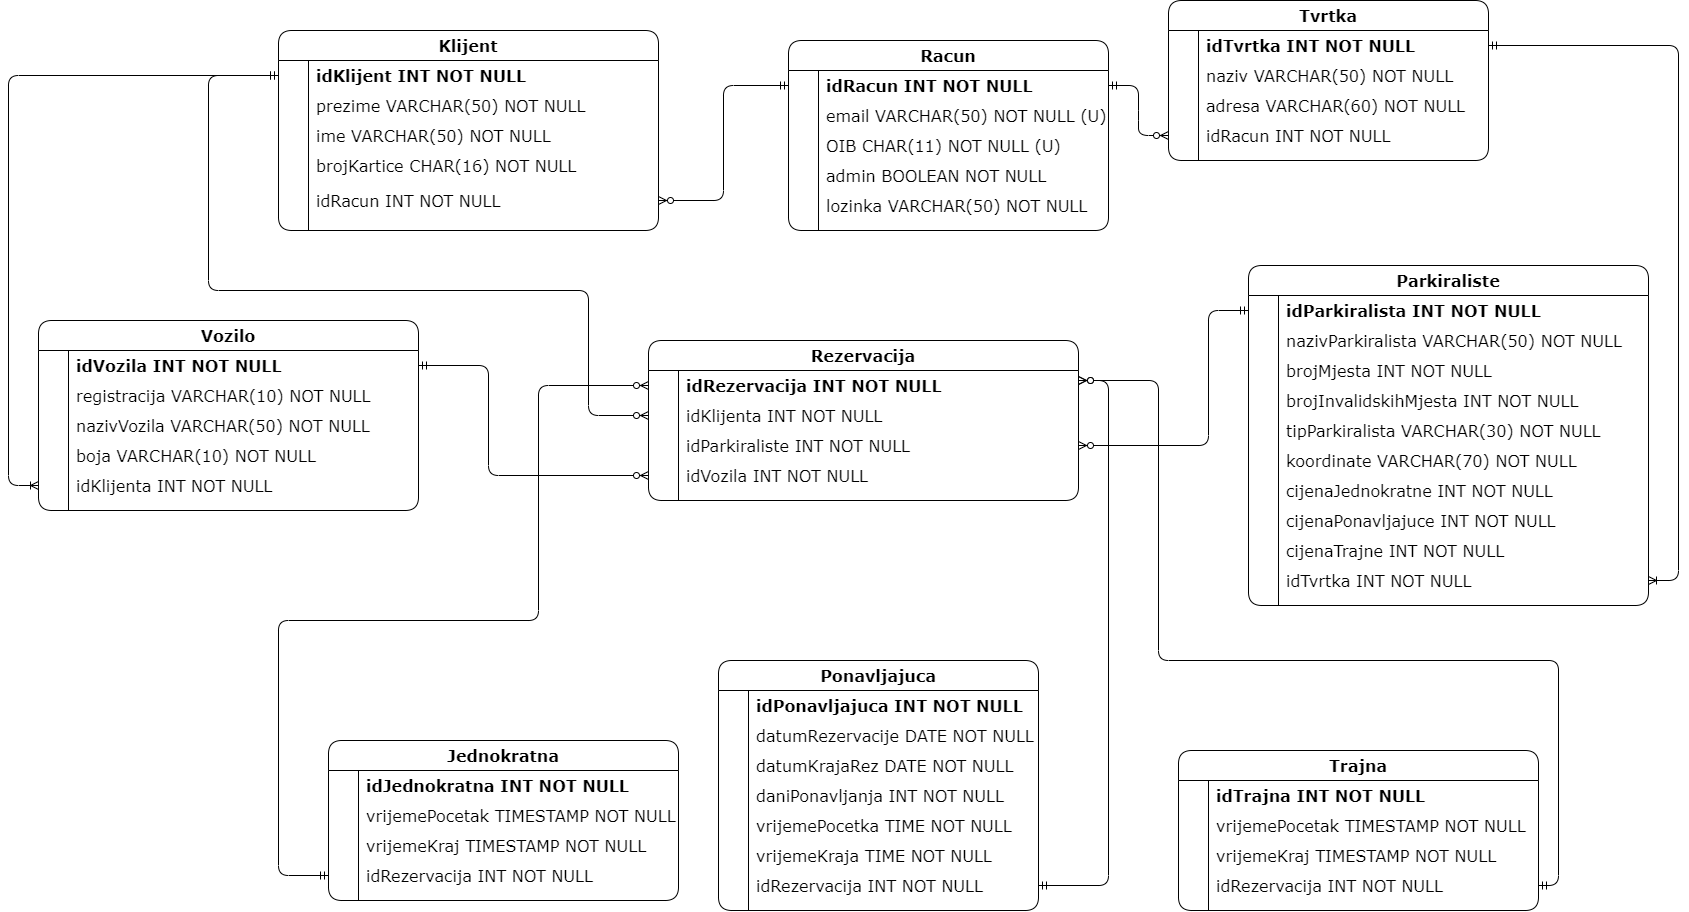
\includegraphics[width=1\linewidth]{dijagrami/ERModel.png} %veličina u odnosu na širinu linije
                	\caption{ER dijagram baze podataka}
                	\label{fig:promjene2} %label mora biti drugaciji za svaku sliku
                \end{figure}
			
			\eject
			
			
		\section{Dijagram razreda}
		
		Na  slikama 4.3, 4.4, 4.5, 4.6, 4.7 prikazani su razredi koji pripadaju \textit{backend} dijelu MVC arhitekture. Razredi na slici 4.3 oponašaju tablice iz baze podataka kojima se pristupa preko ORM-a i pomoću njih se komunicira s bazom podataka. Slika 4.4 prikazuje DTO (\textit{Data transfer object}) razrede koji spremaju podatke kojima kontroleri komuniciraju s \textit{frontend} dijelom aplikacije i modelima. Na slici 4.5 nalaze se razredi koji komuniciraju s bazom podataka i izvršavaju upite koje kontroleri zatraže. Kontroleri su prikazani na slici 4.6. Svi kontroleri nasljeđuju osnovni kontroler koji sadrži metode za slanje odgovora, dok ostali kontroleri nude metode za izvršavanje određenog zahtjeva na određenoj putanji. Slika 4.7 prikazuje jednu vrstu pomoćnih razreda koje smo koristili za prebacivanje podataka iz domene modela u domenu koja se koristi na \textit{frontend} dijelu aplikacije. Postoje još dodatni razredi koji su nebitni za opisivanje rada aplikacije jer služe samo kao pomoćni razredi.
		
		\begin{figure}[H]
	        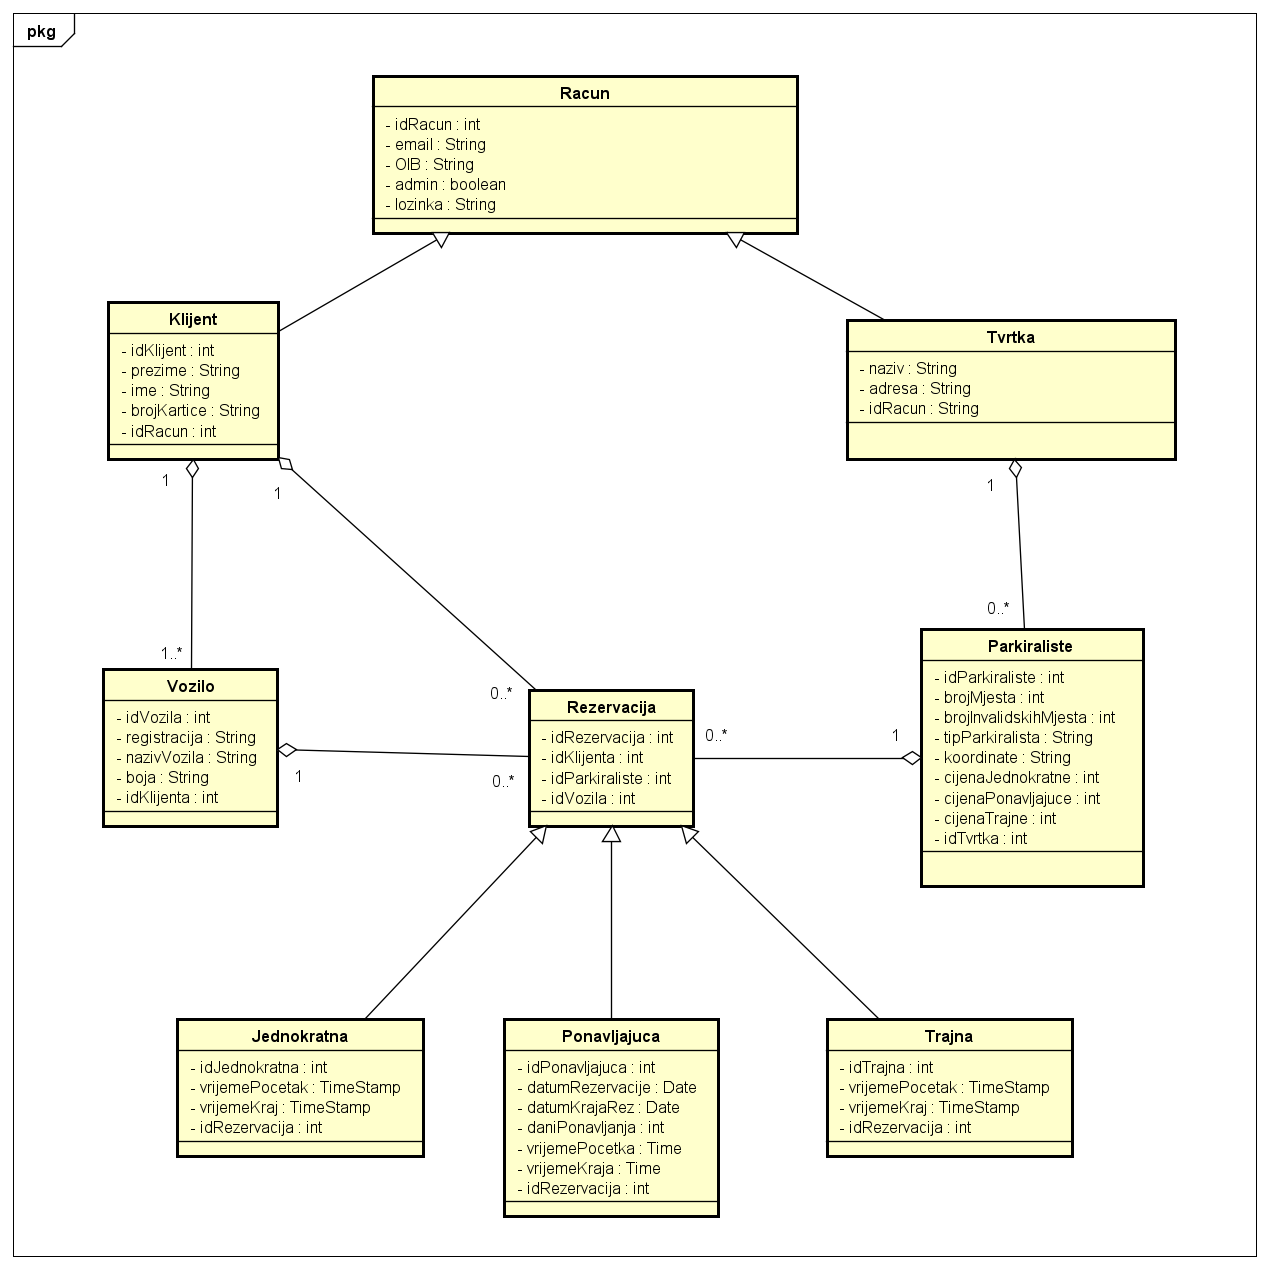
\includegraphics[width=1\linewidth]{dijagrami/Dijagram razreda - Modeli.png}
        	\caption{Dijagram razreda za modele}
        	\label{fig:Dijagram razreda - modeli}
        \end{figure}
    
    	\begin{figure}[H]
	    	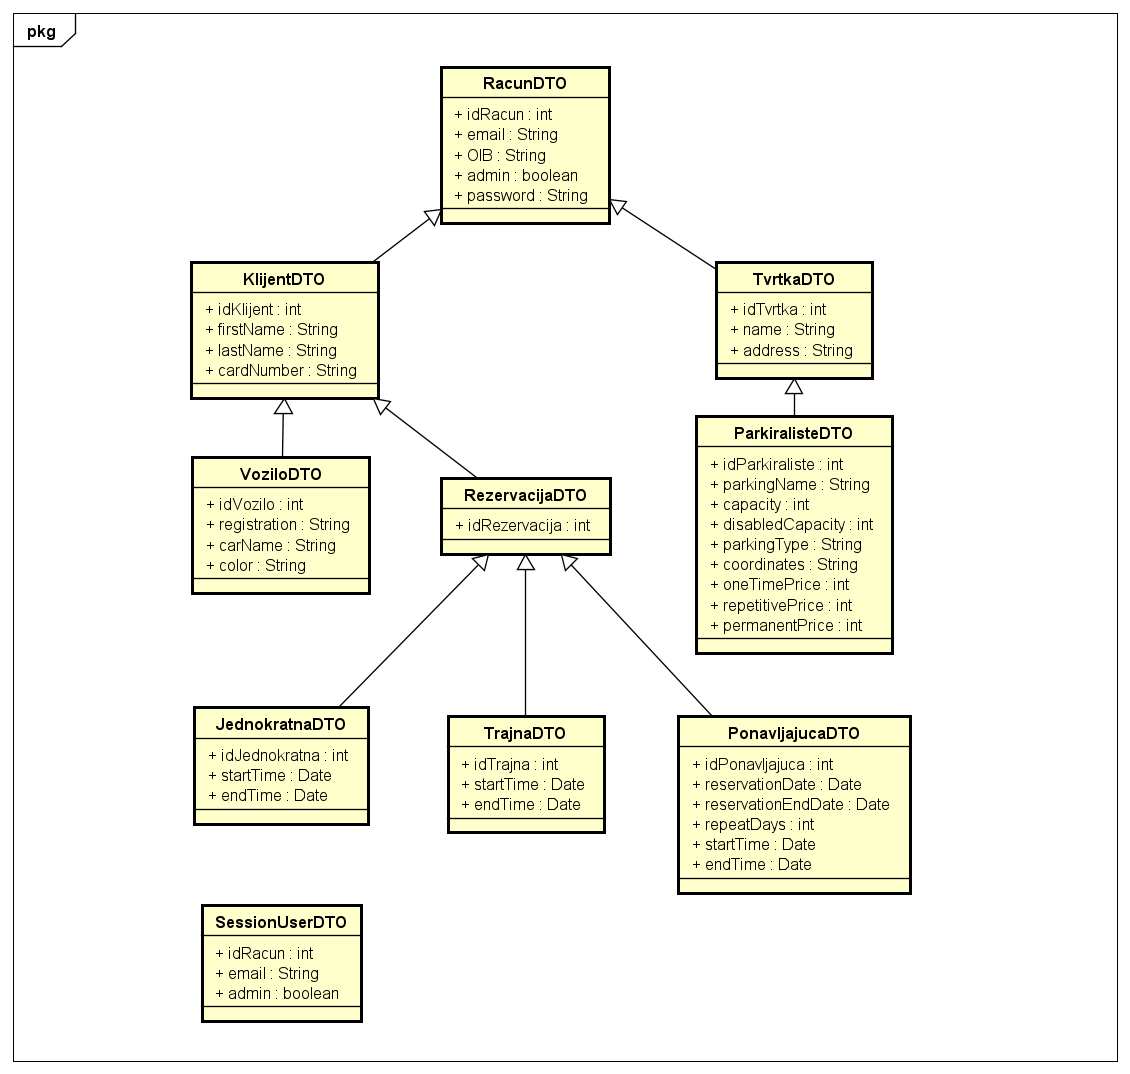
\includegraphics[width=1\linewidth]{dijagrami/Dijagram razreda - DTO.png}
	    	\caption{Dijagram razreda za DTO}
	    	\label{fig:Dijagram razreda - DTO} 
	   	 \end{figure}
    
		\begin{figure}[H]
			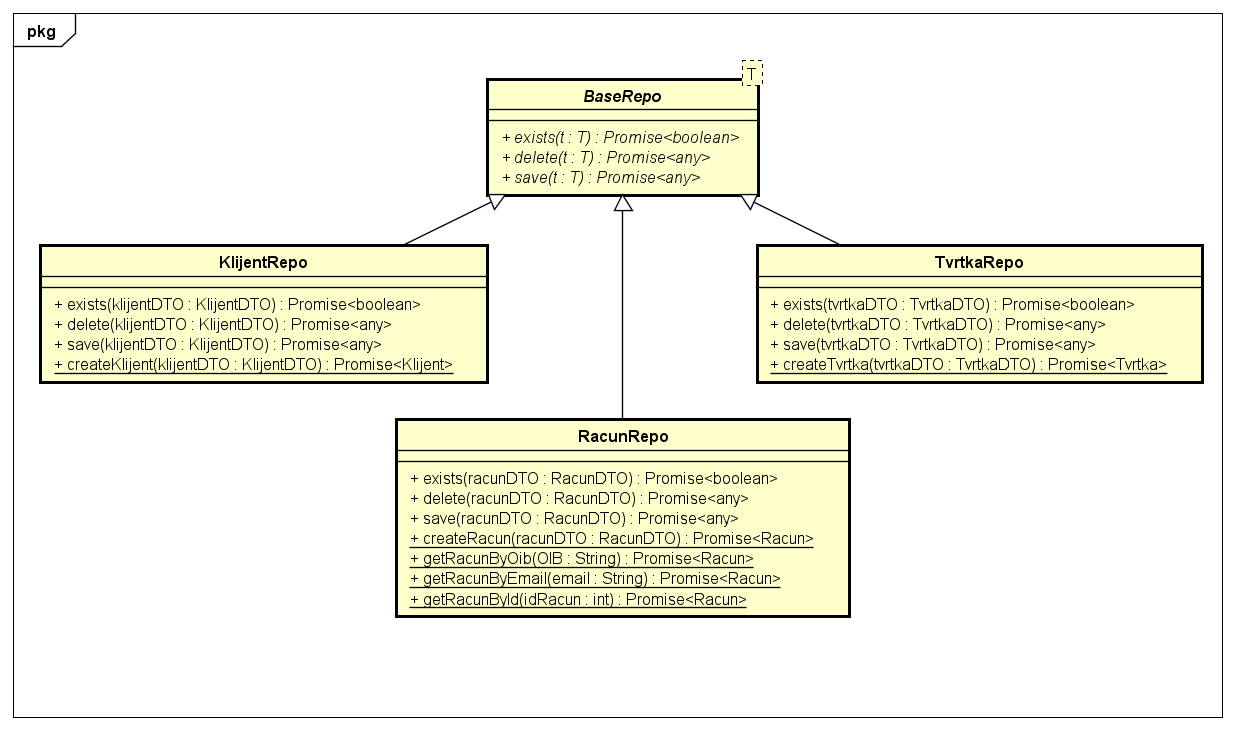
\includegraphics[width=1\linewidth]{dijagrami/Dijagram razreda - Repo.png}
			\caption{Dijagram razreda za repo}
			\label{fig:Dijagram razreda - Repo} 
		\end{figure}
	
		\begin{figure}[H]
			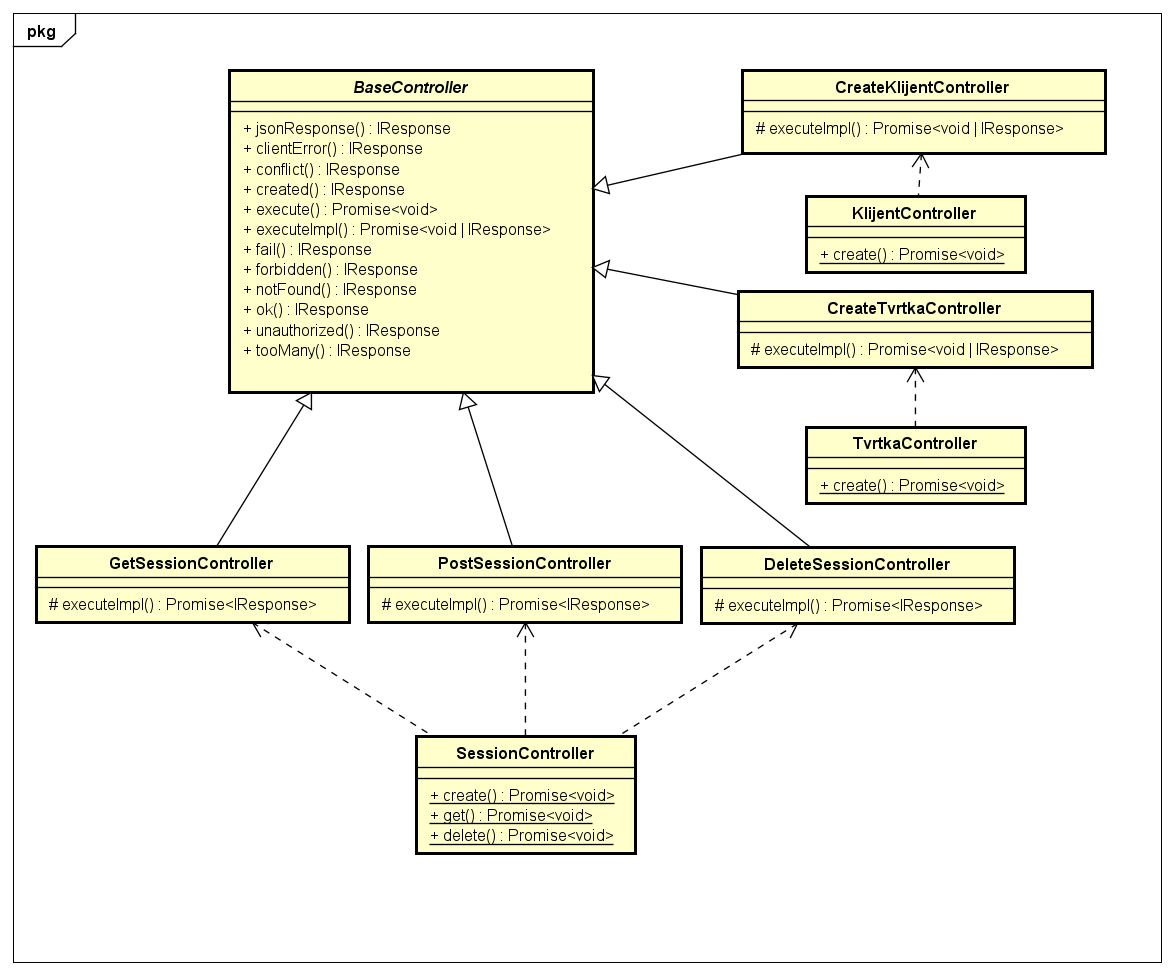
\includegraphics[width=1\linewidth]{dijagrami/Class Diagram - controllers.png}
			\caption{Dijagram razreda za kontrolere}
			\label{fig:Dijagram razreda - Kontroleri} 
		\end{figure}	
		\begin{figure}[H]
			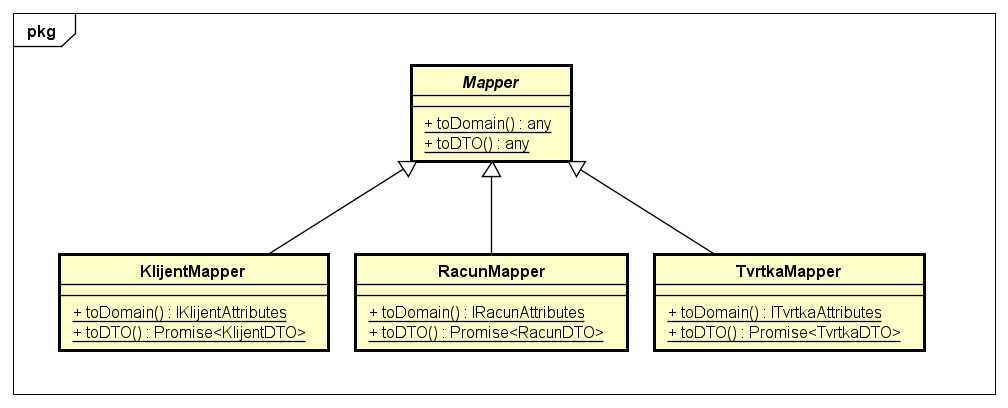
\includegraphics[width=1\linewidth]{dijagrami/Class Diagram - mappers.png}
			\caption{Dijagram razreda za mapere}
			\label{fig:Dijagram razreda - Maperri} 
		\end{figure}
		
			
			\textit{Prilikom prve predaje projekta, potrebno je priložiti potpuno razrađen dijagram razreda vezan uz \textbf{generičku funkcionalnost} sustava. Ostale funkcionalnosti trebaju biti idejno razrađene u dijagramu sa sljedećim komponentama: nazivi razreda, nazivi metoda i vrste pristupa metodama (npr. javni, zaštićeni), nazivi atributa razreda, veze i odnosi između razreda.}\\
			
			\textbf{\textit{dio 2. revizije}}\\			
			
			\textit{Prilikom druge predaje projekta dijagram razreda i opisi moraju odgovarati stvarnom stanju implementacije}
			
			
			
			\eject
		
		\section{Dijagram stanja}
			
			
			\textbf{\textit{dio 2. revizije}}\\
			
			\textit{Potrebno je priložiti dijagram stanja i opisati ga. Dovoljan je jedan dijagram stanja koji prikazuje \textbf{značajan dio funkcionalnosti} sustava. Na primjer, stanja korisničkog sučelja i tijek korištenja neke ključne funkcionalnosti jesu značajan dio sustava, a registracija i prijava nisu. }
			
			
			\eject 
		
		\section{Dijagram aktivnosti}
			
			\textbf{\textit{dio 2. revizije}}\\
			
			 \textit{Potrebno je priložiti dijagram aktivnosti s pripadajućim opisom. Dijagram aktivnosti treba prikazivati značajan dio sustava.}
			
			\eject
		\section{Dijagram komponenti}
		
			\textbf{\textit{dio 2. revizije}}\\
		
			 \textit{Potrebno je priložiti dijagram komponenti s pripadajućim opisom. Dijagram komponenti treba prikazivati strukturu cijele aplikacije.}